    \documentclass{article}
    \usepackage{fancyhdr, amsmath, amsthm, amssymb, mathtools, lastpage, hyperref, enumerate, graphicx, setspace, upgreek}
    \usepackage[margin=1in, top=0.8in,bottom=0.8in]{geometry}
    \usepackage{subcaption}
    \newcommand{\scinot}[2]{#1\times10^{#2}}
    \newcommand{\bra}[1]{\left<#1\right|}
    \newcommand{\ket}[1]{\left|#1\right>}
    \newcommand{\dotp}[2]{\left<#1\,\middle|\,#2\right>}
    \newcommand{\rd}[2]{\frac{\mathrm{d}#1}{\mathrm{d}#2}}
    \newcommand{\pd}[2]{\frac{\partial#1}{\partial#2}}
    \newcommand{\rtd}[2]{\frac{\mathrm{d}^2#1}{\mathrm{d}#2^2}}
    \newcommand{\ptd}[2]{\frac{\partial^2 #1}{\partial#2^2}}
    \newcommand{\norm}[1]{\left|\left|#1\right|\right|}
    \newcommand{\abs}[1]{\left|#1\right|}
    \newcommand{\pvec}[1]{\vec{#1}^{\,\prime}}
    \newcommand{\tensor}[1]{\overleftrightarrow{#1}}
    \let\Re\undefined
    \let\Im\undefined
    \newcommand{\ang}[0]{\text{\AA}}
    \newcommand{\mum}[0]{\upmu \mathrm{m}}
    \DeclareMathOperator{\Re}{Re}
    \DeclareMathOperator{\Tr}{Tr}
    \DeclareMathOperator{\Im}{Im}
    \DeclareMathOperator{\E}{E}
    \DeclareMathOperator{\Var}{Var}
    \newcommand{\expvalue}[1]{\left<#1\right>}
    \usepackage[labelfont=bf, font=scriptsize]{caption}\usepackage{tikz}
	\everymath{\displaystyle}
    \usepackage{listings}

\begin{document}
\title{Ph20.4 - Review: Unix Shell, Make Files, and Version Control}
\author{Cassidy Yang}
\maketitle
\pagestyle{fancy}
\rhead{Cassidy Yang}
\cfoot{Page \thepage \hspace{1pt} of \pageref{LastPage}}

\section{The Assignment - Part I}

For this week's assignment, I created a \texttt{git} repository on github containing all the assignments for Ph20 thus far. The repository can be found at: \texttt{https://github.com/cyang94/ph20.git}.

This is my first time using a git repository, although it seems like a very useful tool for working on projects with other people. I have also included a log of edits made to the repository.

\section{The Assignment - Part II}

For this assignment, I am using the python code modules \texttt{lab1.py} and \texttt{lab2.py}, which are the python scripts written for the first two assignments. \texttt{lab1.py} generates $X(t)$, $Y(t)$, and $Z(t)$ outputs from the first assignment given the necessary input parameters. \texttt{lab2.py} generates a \texttt{.png} image of the convergence rates from the second assignment.

In the makefile, we call \texttt{lab1.py} with the arguments "1 1 1 1 0 0.1 100." We call \texttt{lab2.py}, which generates the following image of the convergence rates. The makefile also compiles and generates this pdf.

\begin{figure}[ht!]
	\centering
	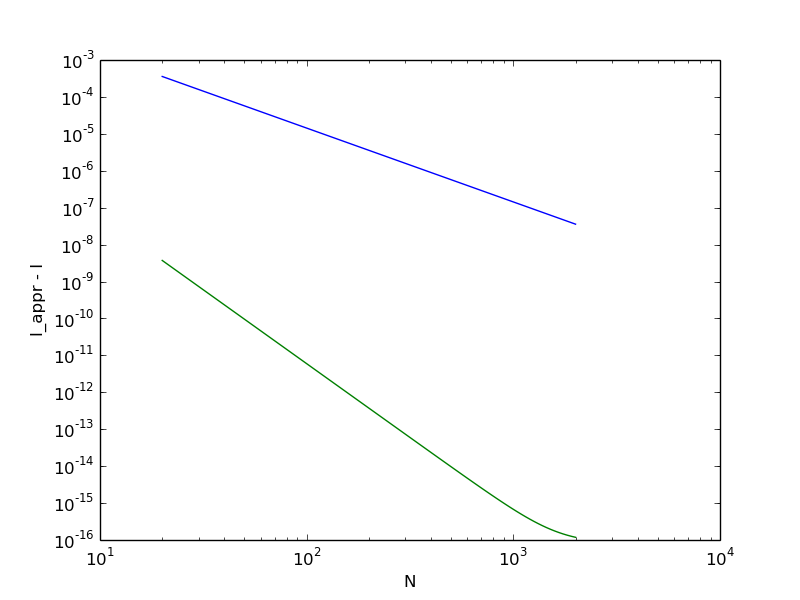
\includegraphics[width=2in]{conv.png}
\end{figure}

The makefile code is attached separately.


\end{document}